\documentclass[14pt]{extarticle}
\usepackage[
left=25mm,
top=20mm,
right=15mm,
bottom=20mm,
]{geometry}

%\usepackage{graphicx}
\usepackage[pdftex]{graphicx}
\usepackage[utf8x]{inputenc}
\usepackage[russian]{babel}
\usepackage[T1]{fontenc}
\usepackage{float}
\usepackage{listings}
\usepackage{cite}
\usepackage{hyperref}
\usepackage{etoolbox}
\usepackage{indentfirst}
\usepackage[linesnumbered,boxed]{algorithm2e}
%\sloppy

\lstset{
	sensitive=true,
	basicstyle=\small,
	keywordstyle=\color{black},
	commentstyle=\scriptsize\rmfamily,
	keywordstyle=\ttfamily\underbar,
	identifierstyle=\ttfamily,
	basewidth={0.5em,0.5em},
	columns=fixed,
	fontadjust=true,
	literate={->}{{$\to$}}1
}

\makeatletter
%\renewcommand{\@biblabel}[1]{#1.} % Заменяем библиографию с квадратных скобок на точку:
\makeatother
\gappto\captionsrussian{\renewcommand{\contentsname}{Оглавление}}
\renewcommand\baselinestretch{1.5}
\renewcommand{\lstlistingname}{Листинг}

\begin{document}
	
	\begin{titlepage}
	\thispagestyle{empty}
		\def\baselinestretch{1.0}
		\begin{center}
			{Правительство Российской Федерации \\ \vskip 0.0em { Федеральное государственное бюджетное образовательное учреждение \\ \vskip 0.0em {высшего профессионального образования \\ \vskip 0.0em { «Санкт-Петербургский государственный университет» \\ \vskip 1.7em{\large Кафедра системного программирования \\}}}}}
			\vspace*{0.05\textheight}
			{\large Гудиев Артур Владимирович}
			
			\vskip 2em
			{\LARGE Реализация примитвов и оконного менеджера для построения пользователских интерфейсов на языке PostScript}
			
			\vskip 1em
			{\large Выпускная квалификационная работа специалиста} \\
			\vskip 2em
			{\normalsize \raggedleft 
				Допущена к защите.\\
				Зав. кафедрой:\\
				д.ф.-м.н., проф. А.Н. Терехов
				\\[2em]
				Научный руководитель:\\
				к.ф.-м.н. Д.Ю. Булычев
				\\[2em]
				Рецензент:\\
				к.ф.-м.н., доц. Д.В. Кознов
				\\[2em]
				%Неизвестно \\
				\vspace*{0.08\textheight}
				{\centering Санкт-Петербург \\ 2015}
			}
		\end{center}
	\end{titlepage}
	\begin{titlepage}
		\thispagestyle{empty}
		\def\baselinestretch{1.0}
		\begin{center}
			{SAINT-PETERSBURG STATE UNIVERSITY \\ \vskip 0.3em {\large Mathematics \& Mechanics Faculty \\ \vskip 0.3em{\large Department of Software Engineering \\}}}
			\vspace*{0.15\textheight}
			{\large Artur Gudiev}
			
			\vskip 2em
			{\LARGE Window manager and GUI primitives for user interface implementation in PostScript}
			
			\vskip 1em
			{\large Graduation Thesis} \\
			\vskip 2em
			{\normalsize \raggedleft 
				Adnitted for defence.\\
				Head of the chair:\\
				professor  Andrey Terekhov
				\\[3em]
				Scientific supervisor:\\
				PhD, Acc. Prof. Dmitri Boulytchev
				\\[3em]
				Reviewer:\\
				PhD, Acc. Prof. Dmitri Koznov
				\\[2em]
				%Неизвестно \\
				\vspace*{0.08\textheight}
				{\centering Saint-Petersburg \\ 2015}
			}
		\end{center}
	\end{titlepage}
	
	\setcounter{page}{3}
	\tableofcontents
	
	%\thispagestyle{empty} 
	\pagebreak
	
	
	\section*{Введение}
	\addcontentsline{toc}{section}{Введение}
	PostScript - это графический интерпретируемый язык программирования, созданный с целью представления графики (текстовых фалов, рисунков, чертежей) в машинонезависимой форме~\cite{PLRM}. С помощью графических операторов языка PostScript можно определить область рисования, отобразить прямые и кривые линии, залить цветом область, задать различные графические параметры.  
	
	Графический интерфейс пользователя является разновидностью пользовательского интерфейса и состоит из различных примитивов - окон, полей ввода, кнопок и т.д. Язык PostScript обладает базовыми возможностями для реализации внешнего вида графических примитивов.
	
	Для полноценной работы графических интерфейсов реализации одних примитивов недостаточно. Требуется также оконный менеджер --- приложение, управляющее размещением примитивов и определяющее их внешний вид. Оконный менеджер позволяет добавлять и удалять примитивы, управлять порядком отображения, пересчитывать координаты и т.д. 
	В оконном менеджере могут быть реализованы также и визуальные эффекты, проявляющиеся во время работы с окнами (например, эффект волны и эффект упорядочивания окон).     
	В каждой операционной системе существует свой оконный менеджер, который взаимодействует с графическими интерфейсами, созданными с помощью, например, Qt~\cite{qtquick} или Swing~\cite{swing}. 
	
	Ранее в рамках проекта лаборатории JetBrains был реализован интерпретатор PostScript~\cite{runtime}~\cite{graphic}~\cite{architecture}. Однако с его помощью было трудно создать графические интерфейсы, а также реализовать оконный менеджер, так как, например, в PostScript не поддерживается механизм обработки событий. Для упрощения реализации этой возможности было решено расширить язык PostScript и на его основе разработать графическую библиотеку, позволяющую создавать графические интерфейсы. Данную работу можно разделить на три направления: оптимизация интерпретатора (Д. Поздин), обработка событий (Р. Макулов) и реализация графических примитивов и оконного менеджера (А. Гудиев). То, что интерпретатор PostScript реализован на языке Java, делает создаваемые им интерфейсы кроссплатформенными.
	
	Целью данной дипломной работы является реализация графических примитивов и оконного менеджера на языке PostScript для решения задачи реализации кроссплатформенных пользовательских интерфейсов.
	
	\pagebreak
	\section{Обзор}
	\subsection{ Описание существующих решений }
		\subsubsection*{Qt Quick}
		%\label{sec:qtquick}
		%\addcontentsline{toc}{subsubsection}{\nameref{sec:qtquick}}

Qt --- это кроссплатформенный фреймворк для создания программного обеспечения, написанный на языке C++.  Qt Quick является средой разработки пользовательских интерфейсов, расспространяемой вместе с Qt. Qt Quick состоит из декларативного языка QML и стандартной библиотеки компонентов QtQuick.
В Qt Quick реализована новая концепция логики моделирования приложений, основанная на иерархической машине состояний\cite{qtquick}. Кроме того, богатый набор анимаций (tweens) облегчают создание полнофункциональных пользовательских интерфейсов.

Как предметно-ориентированная среда разработки она специально ориентирована на создание пользовательских интерфейсов. В Qt Quick нет проблем с приведением типов, указателями и временем жизни объектов. Вместо этого, в центре внимания находится создание богатых пользовательских интерфейсов.

К недостаткам Qt Quick можно отнести необходимость перекомпиляции одной программы для разных платформ. 
		 		
		
		\subsubsection*{Swing}
	    %\label{sec:javaswing}
		%\addcontentsline{toc}{subsubsection}{\nameref{sec:javaswing}}
				
				Компания Sun разработала набор графических компонентов под названием Swing ~\cite{swing}. Компоненты Swing полностью написаны на Java. Для отрисовки используется 2D - API для рисования двумерной графики на языке Java. В Swing легко создавать новые компоненты.

Благодаря простоте использования, детальной документации и гибкости архитектуры Swing стал, пожалуй, самым популярным графическим фреймворком для Java. На его основе создано появилось много расширений, таких как SwingX~\cite{swingx}, JGoodies~\cite{jgoodies}, которые значительно упрощают создание сложных пользовательских интерфейсов. Практически все популярные среды программирования Java включают графические редакторы для Swing-форм, что облегчает освоение Swing.
		
Особенность Swing заключается в том, что приложения Swing могут выглядеть одинаково и по-разному на различных платформах. Приложения, которые внешне одинаково отображаются в разных операционных системах, относительно медленно работают. 
		
		%\label{sec:decisions}
		%\addcontentsline{toc}{subsubsection}{\nameref{sec:decisions}}
	
		
		 
	\subsection{Описание используемых инструментов }
		
		\subsubsection*{JVM}
		%\label{sec:jvm}
		%\addcontentsline{toc}{subsubsection}{\nameref{sec:jvm}}
	
		Виртуальная машина Java (сокращенно JVM) - основная часть среды выполнения для Java, так называемой Java Runtime Environment (JRE). Программы на языке Java компилятором Java (javac) переводятся в байт-код Java. Виртуальная машина Java исполняет байт-код. В настоящее время JVM получила широкое распространение. Ее реализация есть для многих операционных систем, что делает программы, написанные на Java, кроссплатформенными. Интерпретатор PostScript, реализованный в рамках проекта JetBrains, написан на языке Java.
		\subsubsection*{Swing и AWT}
		%\label{sec:swingawt}
		%\addcontentsline{toc}{subsubsection}{\nameref{sec:swingawt}}
		Swing и AWT --- это библиотеки языка Java, с помощью которых в реализованном интерпретаторе строится путь рисования, отображаются шрифты, задаются параметры графической среды исполнения такие, как цвет, ширина линии, способы соединения отрезков и рисования концов отрезка. 
		\subsubsection*{ Интерпретатор PostScript }
		%\label{sec:interpreter}
		%\addcontentsline{toc}{subsubsection}{\nameref{sec:interpreter}}
		Интерпретатор PostScript, реализованный в рамках проекта JetBrains, написан на Java. Он состоит из следующих пакетов: парсер (parser), среда исполнения (runtime) и интерпретатор (interpreter). 
		
		Парсер разбивает входной поток на токены согласно синтаксису PostScript и записывает их в виде процедуры.
		
		Среда исполнения содержит в себе реализацию основных операторов (таких как add, if, for, show ...) и объектов, то есть их значений, типов и атрибутов. Среда исполнения содержит также и класс AVL-дерева, используемый в словарях, стеки, виртуальную память, в которой хранятся значения сложных объектов и графическую среду исполнения. В графической среде исполнения описаны классы отображения результата программы на экране, матрица преобразования системы координат, класс пути, с помощью которого строится изображение, класс снимка графического состояния, используемый при сохранении или восстановлении графического состояния и набор графических параметров (таких как цвет, ширина линии, форма концов отрезка ... ).
		
		Интерпретатор передает парсеру программу PostScript, получает в качестве результата процедуру, кладет ее на стек исполнения и запускает выполнение стека исполнения.
		
	\subsection{ Проект по разработке графической библиотеки PostScript }
Задача реализации интерпретатора графического языка PostScript решается в рамках проекта лаборатории JetBrains. Одно из назначений библиотеки --- создание кроссплатформенных пользователских интерфейсов.
		
		Текущую деятельность в проекте можно разделить на следующие задачи:
		\begin{itemize}
		\item оптимизация интерпретатора;
		\item добавление механизма обработки событий;
		\item реализация примитивов и оконного менеджера.
		\end{itemize}	
	
	В языке PostScript нет механизма обработки событий, что осложняет создание интерфейсов. Поэтому было решено расширить язык PostScript, добавив в него новые операторы, и, используя средства языка Java, реализовать поддержку событий. Используя механизм событий, требуется реализовать графические примитивы (окно, поле ввода, кнопка и т.д.) и оконный менеджер. Примитивы должны отображаться на экране средствами языка PoscScript. Кроме того, необходимо, чтобы при возникновении событий у примитивов исполнялись заданные процедуры. Требуется также, чтобы оконный менеджер управлял порядком отображения примитивов, их добавлением и удалением, пересчетом координат, перерисовкой и т.д. Использование в программе механизма обработки событий, графических примитивов и оконного менеджера может существенно замедлить исполнение программы, поэтому для полноценной работы создаваемых интерфейсов необходима оптимизация интерпретатора.
	\pagebreak
	\section{Реализация графических примитивов}
	В данной главе описывается сначала общая внутренняя структура примитивов, а затем особенности каждого примитива.
	\subsection{Структура примитивов}
		Код графческой библиотеки языка PostScript содержится в файле  glib.ps. В нем создается словарь gelements. У каждого примитива есть свой номер, по которому он хранится в словаре gelements. 
		
		У графических примитивов реализовано отношение наследования. Общий предок у всех --- объект сцена (scene). У каждого примитива есть дети-примитивы. Номера детей хранятся в поле-массиве children.
		
		Каждому графическому примитиву соответствуют два файла --- файл с описанием объекта и файл с процедурой отрисовки примитива (например, для кнопки --- это button.ps и paintButton.ps). 
		
		В файле первом есть два конструктора --- абсолютный и относительный. У каждого примитива есть свои координаты и размеры. Если координаты задаются относительно родителя, то вызывается относительный контсркутор. Если примитив задается абсолютными координатами, тогда вызывается абсолютный. Например, пусть есть окно с левым нижним концом в точке (0,0), высотой 1000 и шириной 1000. Пусть от окна наследуется кнопка с левым нижним концом в (200, 300), длиной 400 и шириной 500. 
		Тогда абсолютный контсруктор будет вызываться с параметрами 200, 300, 400 и 500. 
А относительный --- с 0.2, 0.3, 0.4 и 0.5.
Относительные координаты полезны тем, что при изменении размеров или сдвиге родителя, они не изменяются.

Каждому примитиву можно добавить событие - процедуру PostScript. Их может быть несколько. У каждого графического объекта есть словарь eventProcDict, в нем хранятся процедуры, которые вызываются при событии у объекта. 

	\pagebreak
	\subsection{Примитивы графической библиотеки}
	%\label{sec:button}
	%\addcontentsline{toc}{subsection}{\nameref{sec:button}}
	\textbf{Кнопка} --- это примитив, у которого вызывается заданное событие по нажатию. У кнопки есть два варианта отрисовки: с обычной и с нажатой кнопкой. В процедуре рисования проверяется, нажата ли кнопка. Если да, то рисуется затемненная кнопка без тени (см. рис. ~\ref{button2}), а иначе светлая с тенью (см. рис. ~\ref{button1}) .
	\vskip 1em
		\begin{figure}[h!]
		\begin{center}
		\begin{minipage}[h]{0.4\linewidth}
		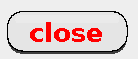
\includegraphics[width=180pt]{pictures/close1.png}
		\caption{ Кнопка} %% подпись к рисунку
		\label{button1} %% метка рисунка для ссылки на него
		\end{minipage}
		\hfill 
		\begin{minipage}[h!]{0.4\linewidth}
		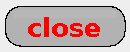
\includegraphics[width=180pt]{pictures/close2.png}
		\caption{Нажатая кнопка}
		\label{button2}
		\end{minipage}
		\end{center}
		\end{figure}	
	
		
	%\subsection*{Флажок}
	Примитив \textbf{флажок} позволяет вызывать заданные процедуры при снятии и задании флага. В процедуре отрисовки проверяется, стоит ли флаг. Если стоит, то рисуется галочка в закрашенной области (см. рис. ~\ref{checkbox2}), а иначе отображается пустая область (см. рис. ~\ref{checkbox1}).
	\vskip 1em
		\begin{figure}[h]
		\begin{center}
		\begin{minipage}[h]{0.4\linewidth}
		
\includegraphics[width=150pt]{pictures/checkBox1.png}
		\caption{Флажок} %% подпись к рисунку
		\label{checkbox1} %% метка рисунка для ссылки на него
		\end{minipage}
		\hfill 
		\begin{minipage}[h]{0.4\linewidth}
		
\includegraphics[width=150pt]{pictures/checkBox2.png}
		\caption{Отмеченный флажок}
		\label{checkbox2}
		\end{minipage}
		\end{center}
		\end{figure}	
			
		
	\pagebreak		
	%\subsection*{Поле со списком}
	Примитив \textbf{поле со списком }позволяет выбрать один из заданных вариантов. Данный примитив состоит из поля, в котором отображается выбранный вариант, и списка со всеми вариантами. Изначально список свернут, отображается только поле (см. рис. ~\ref{combobox1}). При нажатии на поле список раскрывается, отображаются все варианты (см. рис. ~\ref{combobox2}). При следующем нажатии по координатам клика проверяется, был ли выбран какой-нибудь вариант, и если да, то вычисляется, какой именно. После этого список сворачивается, и в поле отображается новый вариант. 
	
		\begin{figure}[h!]
		\begin{center}
		\begin{minipage}[h]{0.4\linewidth}
		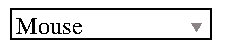
\includegraphics[width=180pt]{pictures/comboBox1.png}
		\caption{ Поле со списком} %% подпись к рисунку
		\label{combobox1} %% метка рисунка для ссылки на него
		\end{minipage}
		\hfill 
		\begin{minipage}[h!]{0.4\linewidth}
		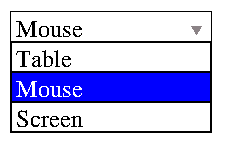
\includegraphics[width=180pt]{pictures/comboBox2.png}
		\caption{Раскрытое поле со списком}
		\label{combobox2}
		\end{minipage}
		\end{center}
		\end{figure}
		
	%\subsection*{Список}
	\textbf{Список} также предоставляет возможность выбора одного из имеющихся вариантов. Отличие списка от поля со списком в том, что в первом список всегда развернут, то есть все варианты постоянно отображаются (см. рис. ~\ref{listbox}). Выбранный вариант рисуется на синем фоне. При нажатии на список проверяется, на каком варианте произошел клик. Затем старый выбранный вариант уже отображается на белом фоне, а новый выбранный - на синем. 
		\begin{figure}[h]
		\center{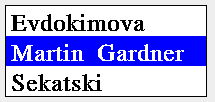
\includegraphics[width=180pt]{pictures/listBox.png}}
		\caption{Список}
		\label{listbox}
		\end{figure}	
	
	%\subsection*{Метка}
		\textbf{Метка} - это примитив, который отображает текст на экране (см. рис. ~\ref{labelField}). При необходимости можно самостоятельно задать размер шрифта и цвет. Для этого нужно в словаре метки поставить по ключу isAttached значение true, и задать необходимые значения ключам kegel и color. 
		\begin{figure}[h]
		\center{
\includegraphics[width=180pt]{pictures/label.png}}
		\caption{ Метка }
		\label{labelField}
		\end{figure}	

	%\subsection*{Поле редактирования}
	%\label{sec:textField}
	%\addcontentsline{toc}{subsection}{\nameref{sec:textField}}
		Примитив \textbf{поле редактирования} предназначен для ввода текста. Изначально в поле ничего не отображается. При нажатии на поле, появляется курсор. Сразу после ввода символы появляются на экране. Курсор можно сдвигать влево и вправо, в начало и конец строки. Напечатанные символы можно удалять. Если введенная строка превышает ширину поля, то вычисляется, какая подстрока отображается на экране (см. рис. ~\ref{textField}).
		\begin{figure}[h!]
		\center{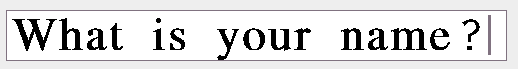
\includegraphics[width=180pt]{pictures/textField.png}}
		\caption{ Поле редактирования }
		\label{textField}
		\end{figure}	
		
		
	%\subsection*{Радиокнопка}
		\textbf{Радиокнопка} - это примитив, который может находиться в включенном или выключенном состоянии. При отрисовке радиокнопки проверяется, в каком она состоянии, и в зависимости от этого отображается включенная (см. рис. ~\ref{rbOn}) или выключенная радиокнопка (см. рис. ~\ref{rbOff}).
		\begin{figure}[h]
		\begin{center}
		\begin{minipage}[h]{0.4\linewidth}
		
\includegraphics[width=90pt]{pictures/toggleButton1.png}
		\caption{ Включенная радиокнопка} %% подпись к рисунку
		\label{rbOff} %% метка рисунка для ссылки на него
		\end{minipage}
		\hfill 
		\begin{minipage}[h]{0.4\linewidth}
		
\includegraphics[width=90pt]{pictures/toggleButton2.png}
		\caption{Выключенная радиокнопка}
		\label{rbOn}
		\end{minipage}
		\end{center}
		\end{figure}
		
		\pagebreak
	%\subsection*{Окно}
	\textbf{Окно} позволяет хранить и отображать в себе другие примитивы (см. рис. ~\ref{window}). У окна можно динамически изменять размеры. Для этого нужно подвести курсор к границе окна, курсор при этом должен поменяться, затем нажать и расстянуть или сжать окно до нужных размеров. При этом у окон задан минимальный размер, меньше которого сжать не получится. Для изменения курсора был введен новый оператор cursor. Окно также можно и перемещать. Для этого нужно зажать верхнюю область окна, и перенести курсор вместе с окном в нужное место. К окну автоматически добавляются служебные примитивы: метка-надпись в верхней части окна и кнопка закрытия. Кнопка закрытия удаляет из словаря графических притивов gelements само окно и всех его потомков.
			
	\begin{figure}[h!]
		\center{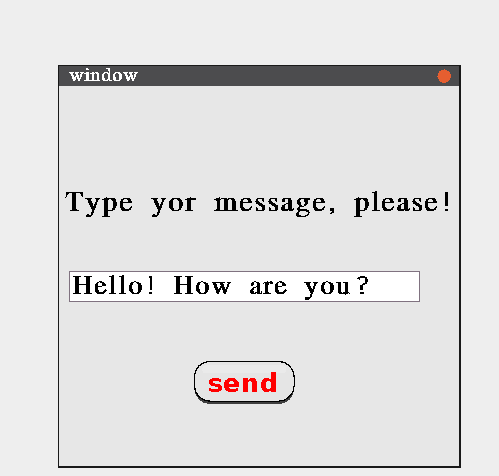
\includegraphics[width=180pt]{pictures/window.png}}
		\caption{ Окно }
		\label{window}
		\end{figure}
	\pagebreak
	
	\section{Оконный менеджер}
	
	В данной главе описаны компоненты, из которых состоит оконный менеджер. Оконный менеджер содержит в себе набор процедур, отвечающих за добавление и удаление примитивов, порядок отображения окон, перемещение и изменение размеров окон, пересчет координат, перерисовку примитивов и визуальные эффекты (см. рис. ~\ref{wmanager}).
	
	\vskip 2em
		\begin{figure}[h]
		\center{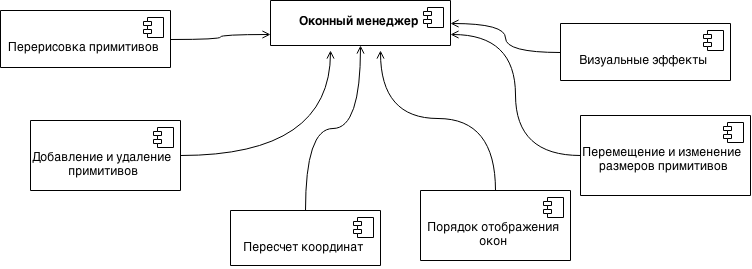
\includegraphics[width=500pt]{pictures/windowManager.png}}
		\caption{ Оконный менеджер }
		\label{wmanager}
		\end{figure}	
	
	\subsection{Добавление и удаление примитивов}
	Для создания примитива нужно вызвать его конструктор с необходимыми параметрами ( расположение, размеры, события...). Конструктор создает словарь, в котором хранятся параметры примитива, и вызывает процедуру \linebreak addElement, которая добавлет примитив-словарь в словарь gelements. Для удаления примитва предназначены продцедуры deleteWithChildren и \linebreak deleteFromParent. deleteWithChildren удаляет сам примитив и всех его потомков из словаря графических примитивов gelements, а deleteFromParent удаляет номер примитива в списке детей у родителя.
	
	\subsection{Порядок отображения окон}
	В программе может быть несколько окон, перекрывающих друг друга. Изначально все окна отображаются в том порядке, в каком они создавались. Но далее, если нажать на произвольное окно, то оно оказывается \textit{в фокусе}. В графической библиотеке glib.ps в словаре gelements создается элемент focusedElement. Изначально это сцена. Но потом при нажатии на произвольный примитив, \linebreak focusedElement становится равным выбранному примитиву. Если на окно нажали, то оно помимо того, что становится в фокусе, ещё и в списке детей родителя ставится последним. Это означает, что оно будет отображаться поверх остальных детей родителя, так как они рисуются в порядке списка.
	
	\subsection{Перемещение и изменение размеров окон}
	Для перемещения и изменения размеров окон в графической библиотеке glib.ps в словаре gelements создаются элементы resizingElement и  draggingElement, отвечающие соответственно за изменение размеров окна и  его перемещение. Изначально они равны null. При нажатии на окно проверяется область нажатия. Если нажата граничная область окна, то resizingElement становится равным данному окну, иначе если нажата верхняя часть окна, то draggingElement оказывается равным нажатому окну. При отпускании окна resizingElement и draggingElement вновь обнуляются.
	
	\subsection{Пересчет координат}
При перемещении или изменении размеров окна, у примитвов-потомков изменяются абсолютные координаты, поэтому их необходимо пересчитывать. За пересчет координат отвечает процедура refreshCoordinatesForChildren. Она у всех детей окна вызывает процедуру refreshCoordinates, которая по своим относительным координатам и абсолютным координатам родителя пересчитывает свои абсолютные координаты. 

\subsection{Перерисовка примитивов}
При некоторых событиях изменяется внешний вид примитивов, поэтому нужна перериосвка. За перерисовку отвечает процедура repaintAll. Она очищает экран с помощью оператора init и запускает с помощью процедуры paintChildren отрисовку всех примитивов, вызывает у каждого примитива процедуру paint. 
		
	\subsection{Визуальные эффекты}
	К примитиву сцене можно добавить процедуры-события для отображения визуальных эффектов. В частности, сейчас добавлено событие волна: при нажатии правой кнопки мыши происходит эффект волны. 
%---------------------4 глава----------------------------------------	
	\pagebreak
	\section{Демонстрационные примеры}
	
	В данной главе приводится описание трех демонстрационных примеров: формы, демонстрации эффектов и калькулятора. На данных примерах тестировались графические примитивы и оконный менеджер, а также их взаимодействие с другими компонентами проекта (например, с механизмом обработки событий).	
	\subsection{Форма}
	
	Ниже приведен демонстрационный пример, содержащий в себе все  реализованные примитивы (см. рис. ~\ref{emptyform}).
	Здесь есть надписи "Welcome!" и "Fill in this form, please."
	За ними идут напдись "Your name" и поле для ввода своего имени.
	Затем метка "Group" и поле для ввода номера своей группы. 
	После этого расположены надпись "Education" и список для выбора формы обучения.
	За формой обучения идут метка "Faculty" и полем со списком для выбора факультета.
	
	Далее флажок с текстом "I want to get results" для подтверждения того, что пользователь хочет получить результат. Если флажок выбран, и  пользователь, заполнив форму (см. рис. ~\ref{filledform}), нажимает кнопку закрытия "Close"\,, то данные с примитивов считываются, записываются в словарь, который затем кладется на стек операндов.
	
	После этого идет надпись "Error checking" и радиокнопка с надписями "On"\, и "Off"\,. Если радиокнопка включена, то при выходе из программы проверяется корректность введенной группы, и если группа введена некорректно, то будет показано окно с ошибкой.	
	Замыкает список примитивов кнопка "Close"\,. При условии успешного прохождения проверки ошибок появляется окно с вопросом, действительно ли пользователь хочет выйти. Если пользователь выбрал кнопку "no"\,, то окно с вопросом просто закрывается. Если же выбрана кнопка "yes"\,, то закрывается вся программа.
	
	\begin{figure}[h]
		\begin{center}
		\begin{minipage}[h]{0.4\linewidth}
		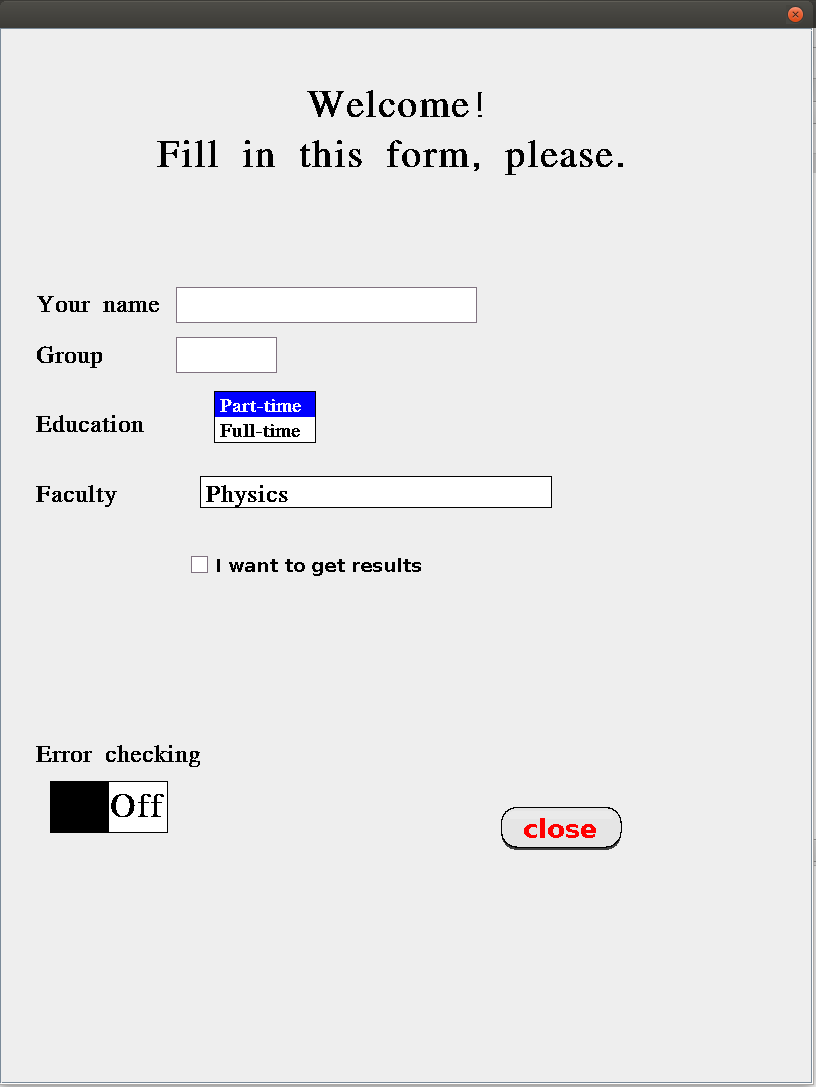
\includegraphics[width=230pt]{pictures/demo11.png}
		\caption{ Пустая форма} %% подпись к рисунку
		\label{emptyform} %% метка рисунка для ссылки на него
		\end{minipage}
		\hfill 
		\begin{minipage}[h]{0.4\linewidth}
		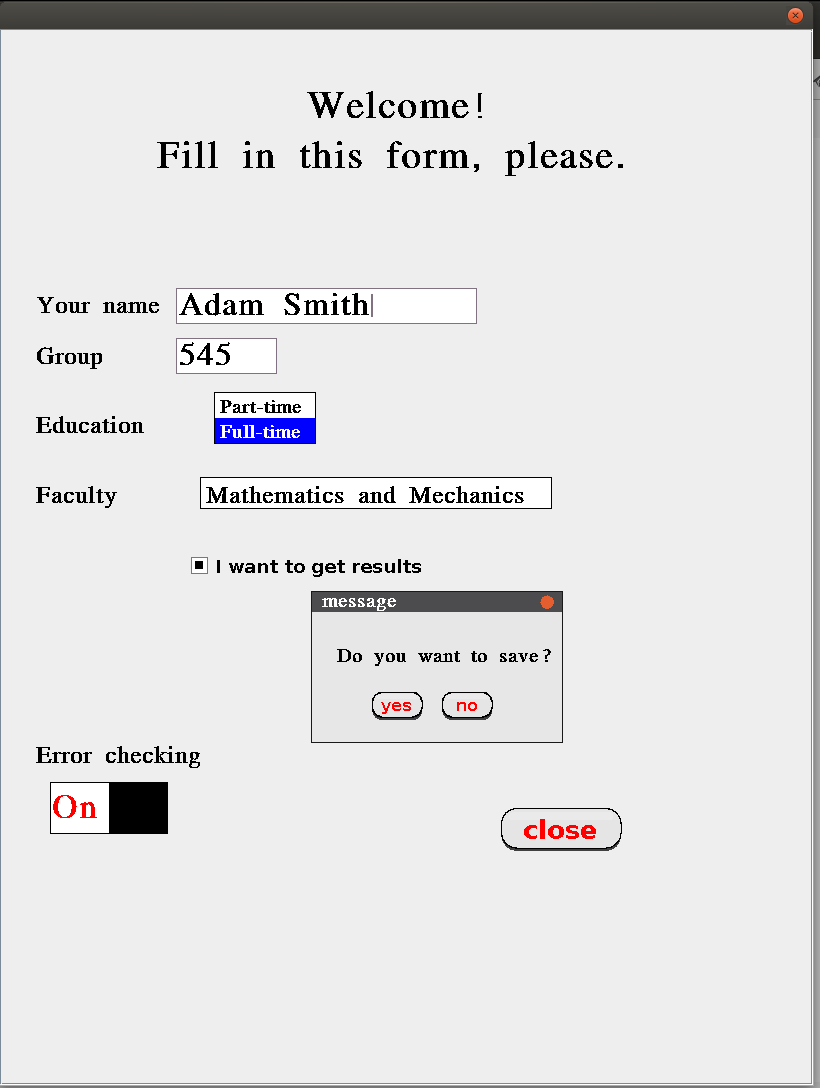
\includegraphics[width=230pt]{pictures/demo12.png}
		\caption{Заполненная форма}
		\label{filledform}
		\end{minipage}
		\end{center}
		\end{figure}
		
		\pagebreak
	Данный пример демонстрирует работу всех примитивов, а также возможность сохранения данных. Кроме того здесь есть создание нового примитива по событию.  
	
	\subsection{Демонстрация эффектов}
	
	В данном демонстрационном примере показывается, как работают различные эффекты, прикрепленные к событиям. 
	Сначала идут надписи "Hello!"\, и "Here you can see various effects"\,.
	За ними идут надпись "scales"\, и кнопки увеличения и уменьшения масштаба.
	Затем метка "translates"\, и четыре кнопки перемещений. 
	Далее расположены надпись "rotates"\, и две кнопки вращения, при нажатии которых происходит поворот (см. рис. ~\ref{rotate}).
	За формой обучения идут метка "reflections"\, и два флажка, включающих эффект отражения.
	Затем  следует надпись "invert labels"\, и кнопка с событием изменения надписей в программе.
	В конце расположена кнопка "Close"\,, закрывающая программу. 
	Кроме того, если нажать правой кнопкой мыши в области интерфейса, то появляется эффект волны (см. рис. ~\ref{wave}). 
	
	\begin{figure}[h]
		\begin{center}
		\begin{minipage}[h]{0.4\linewidth}
		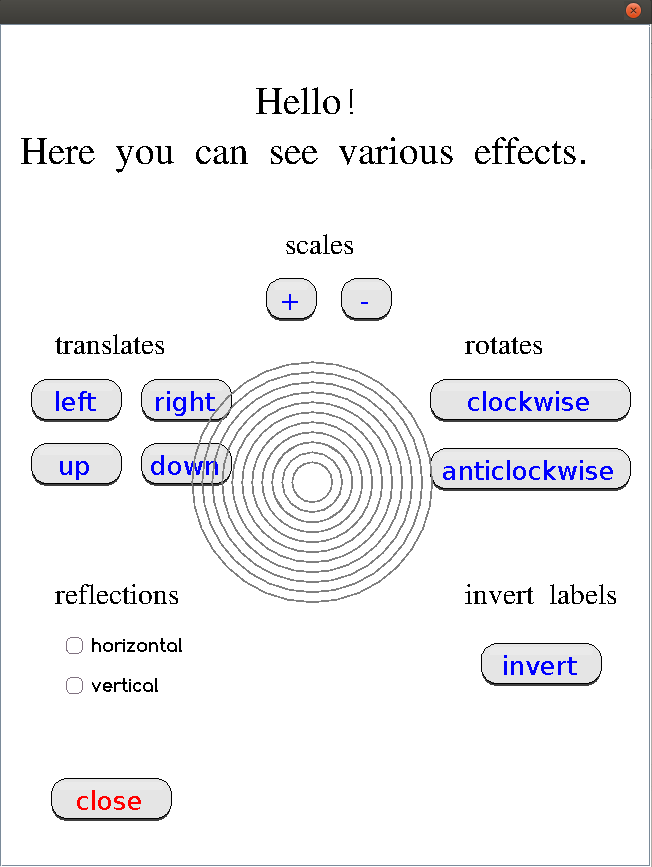
\includegraphics[width=230pt]{pictures/demo21.png}
		\caption{ Эффект волны} %% подпись к рисунку
		\label{wave} %% метка рисунка для ссылки на него
		\end{minipage}
		\hfill 
		\begin{minipage}[h]{0.4\linewidth}
		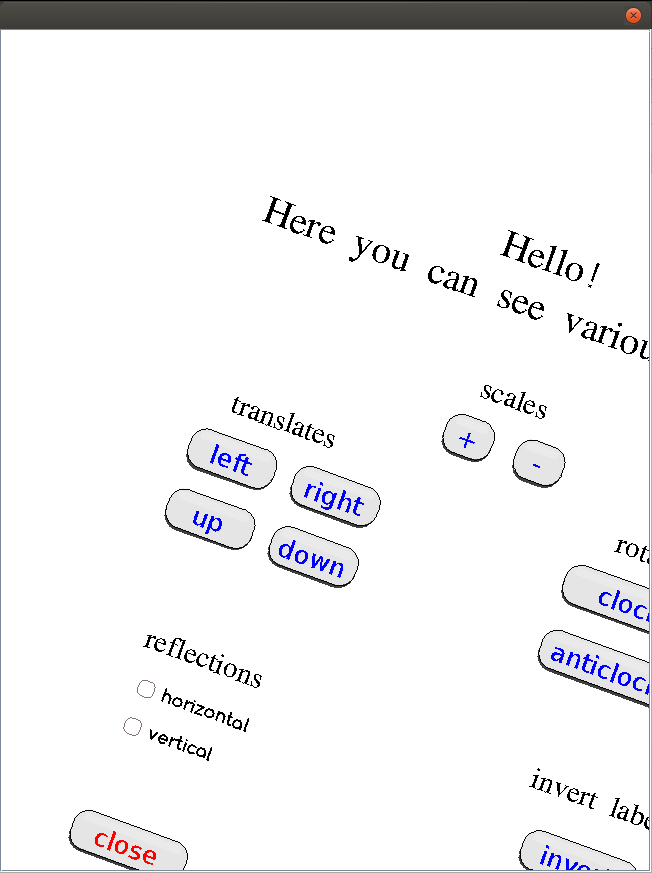
\includegraphics[width=230pt]{pictures/demo23.png}
		\caption{Поворот}
		\label{rotate}
		\end{minipage}
		\end{center}
		
			\end{figure}
		
	Данный пример демонстрирует работу различных преобразований системы координат, а также эффекта волны.  
	
	\subsection{Калькулятор}
	
	Третий пример показывает, как можно не только считывать информацию с примитивов, но изменять их состояния по событиям других примитивов.
	Сначала идут надписи "Welcome!"\, и "You can calculate here"\,.
	Затем идет окно-калькулятор. 
	В нем есть поле для ввода и отображения чисел, кнопка очищения поля, а также кнопки с цифрами, арифметическими операциями, точкой и знаком равно.
	Вычисления выполняется с помощью конечного автомата (см. рис. ~\ref{automate}), в котором есть 4 состояния (1 --- ввод первого числа, 2 --- сохранение первого числа и операции, 3 --- ввод второго числа, 4 --- вывод результата). В программе создается словарь calculator и в нем хранятся состояние, операция и введенные числа. 
		\vskip 1em
		\begin{figure}[h]
		\begin{center}
		\begin{minipage}[h]{0.4\linewidth}
		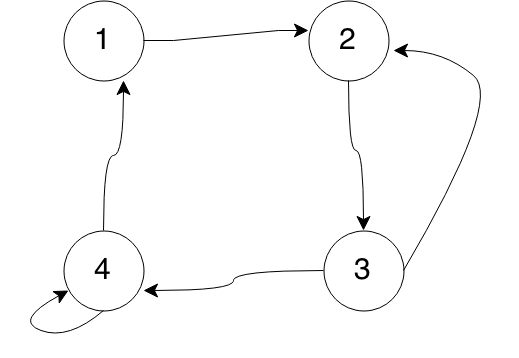
\includegraphics[width=240pt]{pictures/automate.png}
		\caption{ Конечный автомат } %% подпись к рисунку
		\label{automate} %% метка рисунка для ссылки на него
		\end{minipage}
		\end{center}
		\end{figure}
	
	Из третьего состояния можно вернуться во второе, если после ввода второго операнда выбирается новая арифметическая операция. При этом автоматически вычисляется и отображается результат старых операндов, результат сохраняется в качестве первого числа, а второе число не меняется. 
	
	Петля в четвертом состоянии показывает, что если несколько раз нажать знак равенства, то к результату каждый раз будет применяться последняя операция со вторым операндом.
	
	При вычислении результата проверяется, какого тип результат (real или integer). Если это возможно, то идет приведение типов (приведение real к integer). Кроме того, при выводе результата, вычисляется какая подстрока строки будет выведена на экран (с помощью процедуры setTextToTextField).
	
	
	\begin{figure}[h]
		\begin{center}
		\begin{minipage}[h]{0.4\linewidth}
		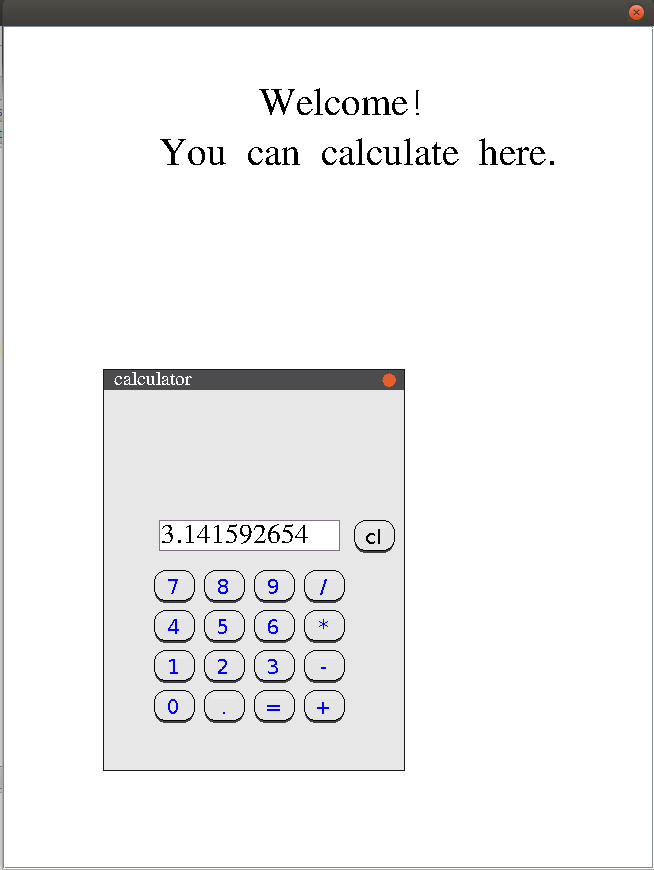
\includegraphics[width=220pt]{pictures/filledCalc.png}
		\caption{ Калькулятор} %% подпись к рисунку
		\label{calculator} %% метка рисунка для ссылки на него
		\end{minipage}
		\end{center}
		\end{figure}
		
	Данный пример демонстрирует сохранение данных и их дальнейшее использование в событиях ( см. рис. ~\ref{calculator}).
	
	\pagebreak
	\section*{Заключение}
	\addcontentsline{toc}{section}{Заключение}
	
	В рамках дипломной работы получены результаты, перечисленные ниже.
	\begin{itemize}
		\item Добавлены следующие примитивы в графическую библиотеку  PostScript: кнопка, флажок, поле со списком, список, метка, поле редактирования, радиокнопка, окно.
		\item Реализован оконный менеджер, интегрированный с графической библиотекой.
		\item Проведено тестирование оконного менеджера на демонстрационном примере.
	\end{itemize}
	

	
	\pagebreak
\bibliographystyle{ugost2008ls}
	\addcontentsline{toc}{section}{Список литературы}
	
	\begin{thebibliography}{}
		
		\bibitem{PLRM}
		Спецификация языка Postscript. PostScript Language reference. \\
		Adobe Systems. 1999\\
		\url{http://www.adobe.com/products/postscript/pdfs/PLRM.pdf}

		\bibitem{runtime}
		Дмитрий Поздин. Реализация общей поддержки времени исполнения для интерпретатора языка PostScript.// Труды лаборатории языковых инструментов. Выпуск 2. 2014. с. 276-296.
		
		\bibitem{graphic}
		Артур Гудиев.
		Реализация графической части интерпретатора языка PostScript.// Труды лаборатории языковых инструментов. Выпуск 2. 2014. с. 297-312.

		\bibitem{architecture}
		Рустам Макулов.
		Архитектура интерпретатора для исполнения программ на языке PostScript в JVM. // Труды лаборатории языковых инструментов. Выпуск 2. 2014. с. 259-275.
				
		\bibitem{qtquick}
		[Qt Developer Network Wiki], 
		\url{https://wiki.qt.io/IntroductionQtQuick/ru}
		
		\bibitem{swing}
		[Хакер], \url{https://xakep.ru/2014/09/10/java-gui/}
		
		
		\bibitem{swingx}
		[The Source for Java Technology Collaboration], \url{https://swingx.java.net/}
		
		
		\bibitem{jgoodies}
		[JGoodies], \url{http://www.jgoodies.com/}
		
	\end{thebibliography}
\end{document}
